% if the names do not fit well on one line use
%         Author 1 \\ {\bf Author 2} \\ ... \\ {\bf Author n} \\
% For authors from different institutions:
% \author{Author 1 \\ Address line \\  ... \\ Address line
%         \And  ... \And
%         Author n \\ Address line \\ ... \\ Address line}
% To start a seperate ``row'' of authors use \AND, as in
% \author{Author 1 \\ Address line \\  ... \\ Address line
%         \AND
%         Author 2 \\ Address line \\ ... \\ Address line \And
%         Author 3 \\ Address line \\ ... \\ Address line}
%\author{Person 1\and Person 3 \and Person 5 \and Person 2\\
%       {tone}@edu.ro}
% \author{First Author \\
%   Affiliation / Address line 1 \\
%   Affiliation / Address line 2 \\
%   Affiliation / Address line 3 \\
%   \texttt{email@domain} \\\And
%   Second Author \\
%   Affiliation / Address line 1 \\
%   Affiliation / Address line 2 \\
%   Affiliation / Address line 3 \\
%   \texttt{email@domain} \\}
%\input{tcilatex}


\documentclass[11pt]{article}
%%%%%%%%%%%%%%%%%%%%%%%%%%%%%%%%%%%%%%%%%%%%%%%%%%%%%%%%%%%%%%%%%%%%%%%%%%%%%%%%%%%%%%%%%%%%%%%%%%%%%%%%%%%%%%%%%%%%%%%%%%%%%%%%%%%%%%%%%%%%%%%%%%%%%%%%%%%%%%%%%%%%%%%%%%%%%%%%%%%%%%%%%%%%%%%%%%%%%%%%%%%%%%%%%%%%%%%%%%%%%%%%%%%%%%%%%%%%%%%%%%%%%%%%%%%%
\usepackage{eurosym}
\usepackage[final]{acl}
\usepackage{times}
\usepackage{latexsym}
\usepackage[T1]{fontenc}
\usepackage{graphicx}
\usepackage[utf8]{inputenc}
\usepackage{microtype}

%TCIDATA{OutputFilter=Latex.dll}
%TCIDATA{Version=5.50.0.2890}
%TCIDATA{<META NAME="SaveForMode" CONTENT="1">}
%TCIDATA{BibliographyScheme=BibTeX}
%TCIDATA{LastRevised=Tuesday, January 11, 2022 14:47:39}
%TCIDATA{<META NAME="GraphicsSave" CONTENT="32">}

\pdfoutput=1
\begin{document}

\title{SemEval 2022: Patronizing and Condescending Language Detection}
\author{Raluca-Andreea G\^inga \And Bogdan Mihai Dobre \And Radu Sielecki \And Tudor Andrei Dumitra\c{s}cu
}
\date{}
\maketitle

\begin{abstract}
This report is part of the SemEval 2022 Workshop, Task 4 - Patronizing and
Condescending Language Detection, trying to find out Patronizing and
Condescendending Language in any form of text. There were used many methods,
varying from simple Machine Learning algorithms applied on bag of words
embeddings until Bert Embeddings and using Neural Networks in order to solve
both the binary classification and multi-label classification as well.
\end{abstract}

\section{Introduction}

The Patronizing and Condescending Language Detection Task is based on the
paper Don't Patronize Me! An annotated Dataset with Patronizing and
Condescending Language Towards Vulnerable Communities (Perez-Almendros et
al., 2020).

The aim of this task is to identify PCL, and to categorize the linguistic
techniques used to express it, specifically when referring to communities
identified as being vulnerable to unfair treatment in the media.

Participants were provided with sentences in context (paragraphs), extracted
from news articles, in which one or several predefined vulnerable
communities are mentioned. The challenge is divided into two subtasks.

\begin{enumerate}
\item Subtask 1: Binary classification. Given a paragraph, a system must
predict whether or not it contains any form of PCL.

\item Subtask 2: Given a paragraph, a system must identify which PCL
categories express the condescension. The PCL taxonomy has been defined
based on previous works on PCL. There are considered the following
categories:
\end{enumerate}

\begin{itemize}
\item Unbalanced power relations.

\item Shallow solution.

\item Presupposition.

\item Authority voice.

\item Metaphor.

\item Compassion.

\item The poorer, the merrier.
\end{itemize}

\section{Background}

The dataset used for this SemEval 2022 task was Don't Patronize Me! dataset,
which contains a suite of sentences that mention some vulnerable communities
and published in media in a lot of English speaking countries. The
paragraphs were manually annotated to show 1) whether the text contains any
kind of PCL, and 2) if it contains PCL, what linguistic techniques
(categories) are used to express the condescension.

The dataset for subtask 1 (binary classification) contained a number of
10.636 paragraphs and 2.792 instances were used for the categories
classification subtask.

In \ref{fig1}, it can be seen that for the first subtask, there are almost
1000 of texts that contain PCL. That means we're dealing with imbalanced
data that we need to solve it. In the next 3 figures (\ref{fig2}, \ref{fig3}%
, \ref{fig4}), it could be noticed the distribution of the most common words
both in the full dataset, but in texts that contain/don't contain PCL as
well.

\begin{figure}[h]
\centering
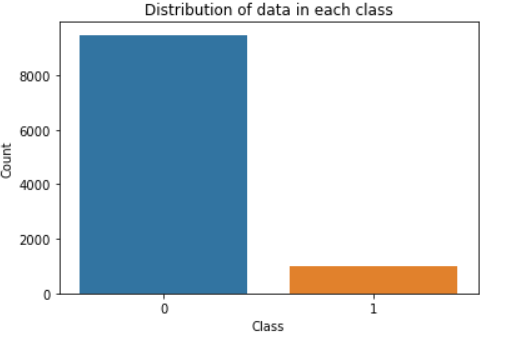
\includegraphics[width=0.5\textwidth]{DataDistribution.png}
\caption{Classes Distribution for Binary Classification problem (Subtask 1)}
\label{fig1}
\end{figure}

\begin{figure}[h]
\centering
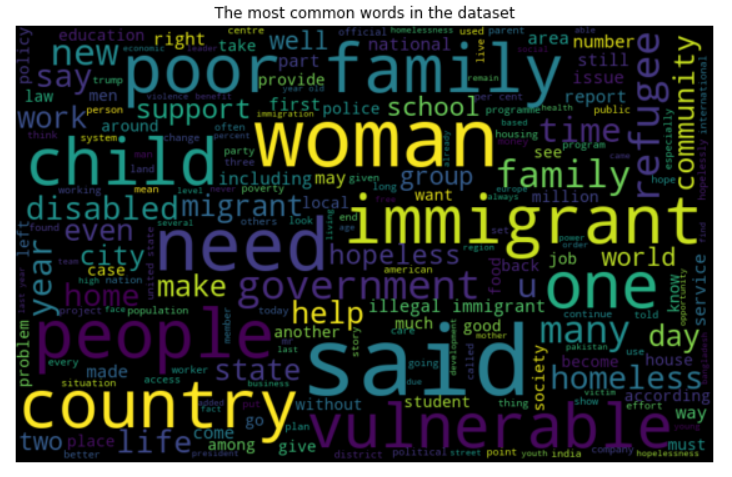
\includegraphics[width=0.5\textwidth]{common.png}
\caption{Most common words in the dataset (Subtask 1)}
\label{fig2}
\end{figure}

\begin{figure}[h]
\centering
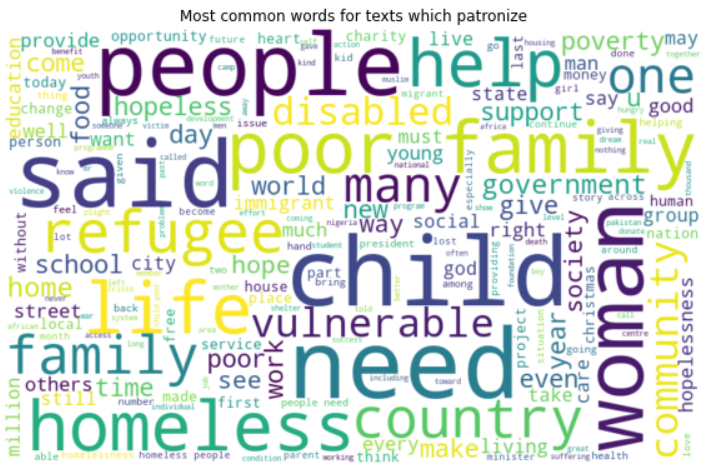
\includegraphics[width=0.5\textwidth]{pcl.png}
\caption{Most common words classified into PCL}
\label{fig3}
\end{figure}

\begin{figure}[h]
\centering
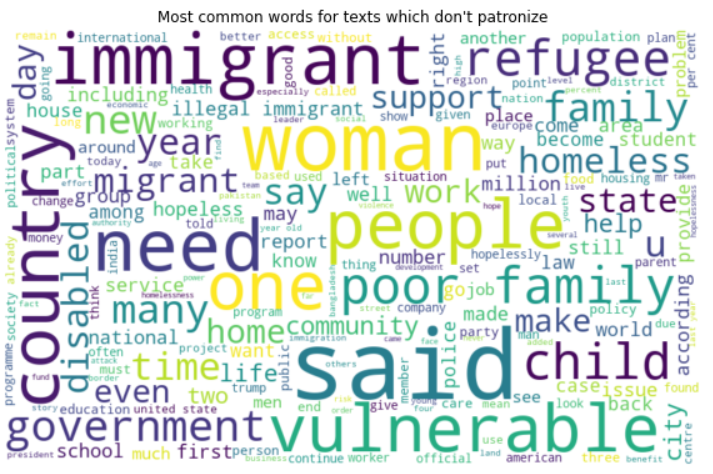
\includegraphics[width=0.5\textwidth]{nopcl.png}
\caption{Most common words of texts that are not PCL}
\label{fig4}
\end{figure}

\section{System Overview}

\begin{enumerate}
\item Subtask 1 (Binary Classification)

Because the dataset was very imbalanced, we tried different approaches in
order to make it balanced:

\begin{itemize}
\item Adding a class weight to the models used. In this approach, we
computed a metric in which we obtained a class weight according to the
imbalance of the dataset. Through this method, we gave some different
weights to both the majority and minority classes. This whole process had
the purpose to penalize the misclassification made by the minority class by
setting a higher class weight and at the same time, reducing the weight for
the majority class.

\item Using oversampling methods and special ensemble techniques. In this
approach, there were used methods like SMOTE (Synthetic Minority
Over-sampling Technique), Adasyn (Adaptive Synthetic), SVM-SMOTE and self
paced ensemble that performs strictly balanced under-sampling in each
iteration, being very efficient computationally.

\item Augmenting the data. Because we notice so little data for label 1, we
decided to collect hate speech datasets and add the positive texts into our
dataset in order to balance the classes frequency, obtaining a total of 6372
from 795 initial texts with label 1. We'll notice in the results section
that this collection and generation of new dataset didn't provide good
results.
\end{itemize}

The dataset was a little bit preprocessed and split into two preprocessed
types: lemmatized cleaned dataset and stemmed cleaned dataset. These two
datasets were generated in order to make some comparison between those two
techniques and to see which provided the best results.

As feature extraction techniques, there were used techniques like Bag of
Words, Tokenizer, Word2Vec and, finally, BertTokenizer which provided the
best results in the end.

As models, there were used Neural Networks with 3 dense layers, Long Short
Term Memory (LSTM) with 64 and 128 neurons with dropout as well, basic
Machine Learning algorithms like Logistic Regression, Random Forest, Support
Vector Machines as XGBoost. In the end, we decided to try BERT embeddings
and a classification BERT model, BertForSequenceClassification, that
contains a single linear classification layer on top and that provided the
best results after all of the other approaches.

Another approach, called "Text shards" made use of the subtask related to
multiclass classification as well. For an average text that contains PCL,
only some small pieces of them are actually PCL and the rest of the text are
not. The assumption is that this confuses the model, because a a combination
of pcl and non pcl is labeled as PCL. To address this, the following
approach is used:

\begin{itemize}
\item negative examples are left as they are

\item each positive example is replaced with the actual pieces of PCL inside
it that we can get from the categories file

\item the positive examples obtained this way are added with the negative
examples to obtain a training dataset

\item all the sentences are cleaned of characters that are not letters and
the words in each sentence are lemmatized

\item a Tensorflow Hub pretrained model called Universal Sentence Encoder is
trained on it

\item for each text that we want to predict, we first use the model on the
whole text to get an initial label

\item a window (of the size of the average length of a cleaned PCL fragment
* 2) is slided through the text and the model is used to predict that
particular substring. If it is labeled as PCL, then we consider the whole
text as PCL.
\end{itemize}

\item Subtask 2 (Multiclass Classification)
\end{enumerate}

\section{Experimental setup}

For both of the subtasks, the organizers from SemEval provided training and
validation datasets: one subset for training purposes and the other one to
validate the results on the training dataset. These practice splits were
provided in order to generate some predictions for the validation dataset
and submit them to the Codalab and familiarize with the format accepted by
Codalab.

For subtask 1, we experimented with a lot of approaches, varrying from
classical Machine Learning algorithms to Deep Learning techniques. The
metric used for evaluation was F1 score. Since we were dealing with
imbalanced dataset, we decided that for this subtask it's better to use F1
Score, which is the main metric used for SemEval 2022 evaluation as well.

The preprocessing step consisted in:

\begin{itemize}
\item clearing the special characters from the dataset

\item lowercasing the texts

\item removing the stopwords

\item removing the words shorter than 3 character

\item lemmatization / stemming - here we used both of these datasets in
order to compare the results between these 2 techniques as well
\end{itemize}

\bigskip

As techniques approached, there were used:

\begin{itemize}
\item Class weight for imbalanced dataset + 3 Dense Layers

This method consisted in creating the class weights corresponding to the
imbalance of the data and provide it to a Neural Network with 3 Dense Layer
with 512 units, 256 units and, finally, 128 units. The activation used for
the final layer was sigmoid and Adam seemed to be the best optimizer among
the other optimizers used in Neural Networks algorithms. This method was
used on a TFIDF lemmatized and stemmed training dataset with 2000 features.

\item Deep Learning for Oversampled dataset

In this approach, there was used the same Neural Network with 3 dense layers
as proposed above, but this time, this neural network was used on
Oversampled datasets using SMOTE, Adasyn, SVM Smote and self paced ensemble
techniques.

\item Tokenization of the lemmatized and stemmed dataset + LSTM neural
network

This time, we used the Tokenizer library from Tensorflow and tokenized all
of the lemmatized and stemmed training datasets with 2000 as maximum of
features. The sequences were then padded into 100 words (we noticed that the
max length of a sentence didn't pass 60-70 words) and we used a LSTM network
with 128 neurons, a Global Max Pool 1D, followed by a Dense with 64 units
with l1 regularizer and a dropout of 0.1.

\item Classical Machine Learning algorithms on both imbalanced and balanced
datasets

In this approach, there were used Logistic Regression, Random Forest,
Support Vector Machines and XGBoost on both imbalanced datasets (but
specifying the class\_weight = 'balanced') and oversampled datasets as well.

\item Word2Vec + LSTM

Word2Vec was used in this approach in order to extract the embedding matrix
of each word from the dataset and feed the LSTM neural network with that
specific embedding.

\item Data augmentation

Because our dataset was very imbalanced and oversampling methods didn't
bring so many good results, we also tried to collect some Hate Speech
datasets with 1 or 0 labels. In order to balance the classes distributiuon,
we decided to add the hate speech texts into our dataset and apply both
logistic regression algorithm, and a deep learning approach as well with 3
dense layers of 512, 256 and 128 units respectively.

\item BERT Transformers + BertForSequenceClassification

The winner of this problem was using BERT transformers for encoding the
texts and using Bert for sequence classification as a model to predict if a
text contains PCL or not.
\end{itemize}

\section{Results}

\begin{enumerate}
\item Subtask 1 (Binary Classification)

\begin{enumerate}
\item Deep Learning / Machine Learning for Imbalanced and Oversampled
dataset
\scalebox{0.5}{
\begin{tabular}[t]{|l|l|l|l|l|l|l|l|l|}
\hline
& \multicolumn{4}{|l|}{Lemmatized (F1\_Score)} & \multicolumn{4}{|l|}{
Stemmed (F1\_Score)} \\ \hline
Approach & Simple & SPE & SMOTE & SVMSMOTE & Simple & SPE & SMOTE & SVMSMOTE
\\ \hline
Neural Networks & 0.27 & - & 0.2823 & 0.3187 & 0.2698 & - & 0.289 & 0.3166
\\ \hline
Logistic Regression & 0.34 & - & 0.35 & 0.35 & 0.35 & - & 0.38 & 0.37 \\
\hline
Random Forest & 0.067 & 0.31 & 0.19 & 0.16 & 0.038 & 0.31 & 0.21 & 0.13 \\
\hline
Support Vector Machines & 0.27 & - & 0.10 & 0.14 & 0.27 & - & 0.14 & 0.20 \\
\hline
XGBoost & 0.15 & - & 0.23 & 0.24 & 0.17 & - & 0.23 & 0.24 \\ \hline
\end{tabular}
}

\item Tokenization of the lemmatized and stemmed dataset / Word2Vec + LSTM
neural network

\scalebox{0.55}{
\begin{tabular}[t]{|l|l|l|l|l|}
\hline
& \multicolumn{2}{|l}{Lemmatized (F1\_Score)} & \multicolumn{2}{|l|}{Stemmed
(F1\_Score)} \\ \hline
Approach & Simple & Word2Vec & Simple & Word2Vec \\ \hline
LSTM (64 neurons) & 0.2693 & 0.2109 & 0.3213 & 0.2093 \\ \hline
LSTM (128 neurons) & 0.2317 & 0.2308 & 0.2789 & 0.2412 \\ \hline
\end{tabular}
}

\item Data augmentation

\scalebox{0.55}{
\begin{tabular}[t]{|l|l|}
\hline
& Augmented Data (F1\_Score) \\ \hline
NNs with 3 layers & 0.2155 \\ \hline
Logistic Regression & 0.23 \\ \hline
Universal Sentence Encoder + 2 dense layers & 0.2316 \\ \hline
\end{tabular}
}

\item BERT Transformers + BertForSequenceClassification

\scalebox{0.55}{
\begin{tabular}[t]{|l|l|}
\hline
& Unprocessed data (F1\_Score) \\ \hline
Bert Tokenizer + Classifier & 0.5074 \\ \hline
\end{tabular}
}
\end{enumerate}

\item Subtask 2 (Multiclass Classification)
\end{enumerate}

\section{Conclusion}

In the current project, it was solved the problem posed by SemEval 2022 Task
4: Patronizing and Condescending Language Detection. There were applied
various methods, including the application of Word Embeddings (Bag of Words,
Word2Vec, BERT), tokenization, oversampling/undersampling of the datasets.
In the binary classification problem, the approach that gave the best result
on the validation dataset was BERT transformers combined with Bert for
Sequence Classification, obtaining 0.50 as f1\_score.

\subsection{References}

\appendix

\section{Example Appendix}

\label{sec:appendix}

This is an appendix.

\end{document}
